A process of decomposing a joint probability distribution is named factorisation. It is performed to obtain a such a set of factors which product is equal to a given joint probability distribution. Therefore, factorisation can largely decrease the complexity of calculations as it is only required to calculate the outcome of each factor within its scope that is usually much smaller than the whole input domain. A base for defining a factor in undirected graphs is a clique which is defined as a subset of nodes in which each variable is connected to every other variable in a set. A clique which is not a subset of any other clique, and therefore cannot be extended by adding any more nodes, is called a maximal clique \cite{clique}. Given an undirected graph $G=(V,\pazocal{E})$ modelled with a set of nodes, also called vertices $V$, and a set of edges $\pazocal{E}$ a family of joint probability distributions can be obtained as a result of the factorisation process. For a single realisation over all random variables in a model that is denoted as $y$, a joint probability $p(y)$ is understood as a normalised product of factors $\psi_{c}$ of every clique $c$ from a set of all maximal cliques $C$ found in the graph $G$. This is presented in equation \ref{eq:factorisation_joint_probability}, in which $y_c$ denotes all variables nodes from a given clique $c$.
\begin{equation}
    \label{eq:factorisation_joint_probability}
    p(y)=\frac{1}{Z}\prod_{c\in C}\psi_{c}({y_c})
\end{equation}
In those graphs, factors also called clique potentials, do not represent conditional probability. Instead, they are non-negative functions with a property that values with higher potentials are more probable to occur. Thus, a family of joint probabilities does not need to sum up to 1, and therefore, a normalising constant $Z$ is introduced. This constant, also known as a partition function, is expressed as a summation over joint probabilities of all states $y$ in an overall output domain $\pazocal{Y}$.
\begin{equation}
    Z=\sum_{y\in \pazocal{Y}}\prod_{c\in C}\psi_{c}({y_c}) 
\end{equation}

Such factorisation can be presented on a fully connected graph, however, it is not very convenient for further processing. A far more intuitive way of modelling factorisation of a joint probability distribution is to use factor graphs, which are a type of undirected, probabilistic graphical models. Such graphs contain two kinds of nodes – variable nodes, and factor nodes, with each factor node being connected to variable nodes that depend on it. A sample factor graph created for six random variables is depicted in Figure \ref{fig:factor_graph}, where variable nodes are marked as green circles, and factor nodes as black rectangles. As presented, between every pair of factor and variable nodes there is an edge marked.
\begin{figure}[ht]
    \centering
    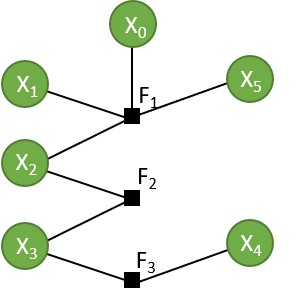
\includegraphics[width=0.5\textwidth]{structured_prediction/factor_graph}
    \caption[Sample scheme of a factor graph.]{Sample scheme of a factor graph with variable nodes marked as green circles and factor nodes as black rectangles.}
     \label{fig:factor_graph}
\end{figure}

Then to calculate joint probability $p(y)$ it is enough to compute a product of each factor $F \in \pazocal{F}$ and normalise it with normalising constant $Z$ as in equations \ref{eq:joint_probability_factor} and \ref{eq:joint_probability_factor_Z}. The scope of the factor $F$ is denoted as $N(F)$ and it represents the set of all variable nodes that are adjacent to this factor.
\begin{align}
    \label{eq:joint_probability_factor}
    p(y) &= \frac{1}{Z}\prod_{F\in \pazocal{F}}\psi_{F}({y_{N(F)}}) \\
    \label{eq:joint_probability_factor_Z}
     Z &=\sum_{y\in \pazocal{Y}}\prod_{F\in \pazocal{F}}\psi_{F}({y_{N(F)}})
\end{align}
Hence, for the sample factor graph from Figure \ref{fig:factor_graph} the joint probability $p(y)$ is equivalent to product of the factor $F_1$ dependent on nodes $x_5, x_0, x_1, x_2$, then the factor $F_2$ with a scope of $x_2, x_3$, and factor $F_3$ which is dependent on $x_3, x_4$, as in equation \ref{eq:joint_probability_example}.
\begin{equation}
    \label{eq:joint_probability_example}
    p(y)=\frac{1}{Z}(\psi_{F_1}(x_5,x_0,x_1,x_2,y_{N(F_1)}) \cdot \psi_{F_2}(x_2,x_3,y_{N(F_2)}) \cdot \psi_{F_3}(x_3,x_4,y_{N(F_3)}))
\end{equation}

For directed graphs it was clear that factors represent conditional probabilities, however, for undirected graphs, the meaning of factors is not so strictly defined. The only requirement for them is to be non-negative as probability cannot be lower than 0. One of the easiest ways of ensuring that factors will output a non-negative value is to present a problem in an exponential domain, which is obtained with the use of energy function. Energy is such a function which exponential represents a factor potential as in equation \ref{eq:energy_definition}.
\begin{equation}
    \label{eq:energy_definition}
    \psi_{F}(y_{N(F)}) = \exp{\Big(-E_F(y_{N(F)})\Big)}
\end{equation}
Then, the joint probability $p(y)$ can be expressed as a summation of energies for each factor as in formula \ref{eq:joint_probability_distribution_factors}.
\begin{equation}
\begin{aligned}
    \label{eq:joint_probability_distribution_factors}
     p(y) &=\frac{1}{Z}\prod_{F\in \pazocal{F}}\bigg(\exp\Big({-E_F(y_{N(F)})}\Big)\bigg) \\
     & =\frac{1}{Z}\exp\bigg(-\sum_{F \in \pazocal{F}}{E_F(y_{N(F)})}\bigg)
\end{aligned}
\end{equation}
For the presented calculations, the normalising constant $Z$ has the following form:
\begin{equation}
    Z=\sum_{y\in \pazocal{Y}}\exp\bigg(-\sum_{F \in \pazocal{F}}{E_F(y_{N(F)})\bigg)}
\end{equation}

Similarly to a factor potential, energy represents how accurate is a given solution \cite{factor_graphs_chopra}. The evaluation is done by assigning a scalar value to each configuration of random variables with an interpretation that the lower an energy is, the more probable is a given configuration. Then to obtain a state $y \in \pazocal{Y}$ that has the highest probability, it is enough to specify such a configuration which will have the lowest energy, as presented in formula \ref{eq:energy_maximisation}.
\begin{equation}
    \label{eq:energy_maximisation}
    \argmax_{y \in \pazocal{Y}}{p(y)} = \argmin_{y \in \pazocal{Y}} \sum_{F\in \pazocal{F}} {E_f}({y_{N(F)}})
\end{equation}

Factorisation is a highly convenient process for supervised learning in which the number of inputs and possible outputs is extensive, as it largely reduces the complexity of the generated model. Furthermore,  factor graphs increase the efficiency of algorithms further described in this dissertation, which are needed to solve prediction problems. 



